\documentclass[aspectratio=169]{beamer}

% =================================================================
%  Introduction to Computer Programming with C
%  A beginner-friendly Beamer deck (fully self-contained: all
%  figures / flowcharts drawn with TikZ, so it compiles anywhere).
% =================================================================

% -------------------------------------------------
% Theme and packages
% -------------------------------------------------
\usetheme{Madrid}
\usecolortheme{default}

\usepackage{amsmath}
\usepackage{amssymb}
\usepackage{bm}
\usepackage{listings}
\usepackage{tikz}
\usepackage{array}
\usepackage{booktabs}
\usepackage{tabularx}
\usepackage{ragged2e}
\usepackage{xcolor}
\usetikzlibrary{shapes.geometric, arrows.meta, positioning, calc, fit, backgrounds}

% -------------------------------------------------
% Colour palette
% -------------------------------------------------
\definecolor{cAccent}{RGB}{0,102,153}     % teal-blue accent
\definecolor{cBox}{RGB}{28,31,42}          % dark box
\definecolor{cGreen}{RGB}{34,139,34}
\definecolor{cRed}{RGB}{178,34,34}
\definecolor{cOrange}{RGB}{204,102,0}
\definecolor{cPurple}{RGB}{102,45,145}
\definecolor{cGrayBg}{RGB}{245,246,248}
\definecolor{codebg}{RGB}{248,248,244}
\definecolor{codekw}{RGB}{0,0,180}
\definecolor{codecomment}{RGB}{0,130,0}
\definecolor{codestr}{RGB}{170,55,20}

% Beamer colour tweaks (match a Madrid-style accent)
\setbeamercolor{structure}{fg=cAccent}
\setbeamertemplate{frametitle continuation}{%
    \ifnum\insertcontinuationcount>1\space(cont...)\fi
}
\setbeamertemplate{navigation symbols}{}
\setbeamertemplate{caption}[numbered]

% -------------------------------------------------
% Listings style for C code
% -------------------------------------------------
\lstdefinestyle{cstyle}{
    language=C,
    backgroundcolor=\color{codebg},
    basicstyle=\ttfamily\footnotesize,
    keywordstyle=\color{codekw}\bfseries,
    commentstyle=\color{codecomment}\itshape,
    stringstyle=\color{codestr},
    numbers=left,
    numberstyle=\tiny\color{gray},
    numbersep=8pt,
    showstringspaces=false,
    breaklines=true,
    frame=single,
    rulecolor=\color{gray!50},
    tabsize=2,
    columns=fullflexible,
    keepspaces=true,
    literate={~}{{$\sim$}}1
}
\lstset{style=cstyle}

% Handy TikZ flowchart node styles
\tikzset{
    startstop/.style={rectangle, rounded corners=10pt, minimum width=2.4cm, minimum height=0.8cm, text centered, align=center, draw=black, fill=cAccent!25},
    process/.style  ={rectangle, minimum width=2.6cm, minimum height=0.8cm, text centered, align=center, text width=2.8cm, draw=black, fill=blue!8},
    io/.style       ={trapezium, trapezium left angle=70, trapezium right angle=110, minimum width=2.2cm, minimum height=0.8cm, text centered, align=center, draw=black, fill=cOrange!20},
    decision/.style ={diamond, aspect=2, minimum width=2.4cm, minimum height=0.9cm, text centered, text width=2.2cm, draw=black, fill=cGreen!18, inner sep=1pt},
    flowarrow/.style={-{Stealth[length=2.5mm]}, thick},
}

% -------------------------------------------------
% Title information
% -------------------------------------------------
\title[Programming with C]{Introduction to Computer Programming}
\subtitle{Fundamentals of C for Complete Beginners}
\author[Amit Kumar Singh]{}
\institute[]{
    Amit Kumar Singh \\
    \vspace{0.1cm}
    Assistant Professor (ECE) \\
    \vspace{0.05cm}
    School of Naval Architecture and Ocean Engineering\\
    \vspace{0.05cm}
    Indian Maritime University Visakhapatnam Campus, Sabbavaram Mandal\\
    \vspace{0.05cm}
    Visakhapatnam, Andhra Pradesh -- 531~035\\
    \vspace{0.25cm}
    amitkumarsingh@imu.ac.in
}
\date[Programming in C]{\today}

\begin{document}

%------------------------------------------------
\begin{frame}
    \titlepage
\end{frame}

%------------------------------------------------
\begin{frame}{Outline}
    \begin{columns}[T]
        \begin{column}{0.5\textwidth}
            \tableofcontents[hideallsubsections, sections={1-6}]
        \end{column}
        \begin{column}{0.5\textwidth}
            \tableofcontents[hideallsubsections, sections={7-12}]
        \end{column}
    \end{columns}
\end{frame}

% =================================================================
\section{Introduction to Computer Organization}
% =================================================================
\begin{frame}{What is a Computer?}
    \begin{block}{Definition}
        A \textbf{computer} is an electronic machine that accepts \textbf{data} (input),
        processes it according to a set of \textbf{instructions} (a program), and produces
        useful \textbf{information} (output).
    \end{block}
    \vspace{0.3cm}
    \begin{columns}
        \begin{column}{0.6\textwidth}
            \begin{itemize}
                \item It follows the simple cycle:
                \[
                    \textbf{INPUT} \;\rightarrow\; \textbf{PROCESS} \;\rightarrow\; \textbf{OUTPUT}
                \]
                \item It cannot ``think'' --- it only does exactly what the program tells it, very fast and without mistakes.
                \item \emph{Programming} is the art of writing those instructions.
            \end{itemize}
        \end{column}
        \begin{column}{0.4\textwidth}
            \centering
            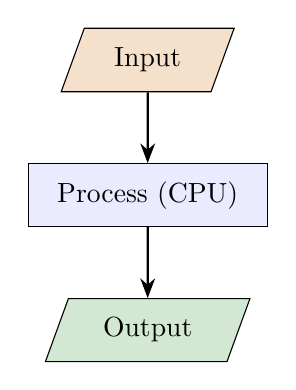
\begin{tikzpicture}[node distance=0.9cm]
                \node[io, fill=cOrange!20] (in) {Input};
                \node[process, below=of in] (proc) {Process (CPU)};
                \node[io, below=of proc, fill=cGreen!20] (out) {Output};
                \draw[flowarrow] (in) -- (proc);
                \draw[flowarrow] (proc) -- (out);
            \end{tikzpicture}
        \end{column}
    \end{columns}
\end{frame}

\begin{frame}{Computer Organization: The Building Blocks}
    \centering
    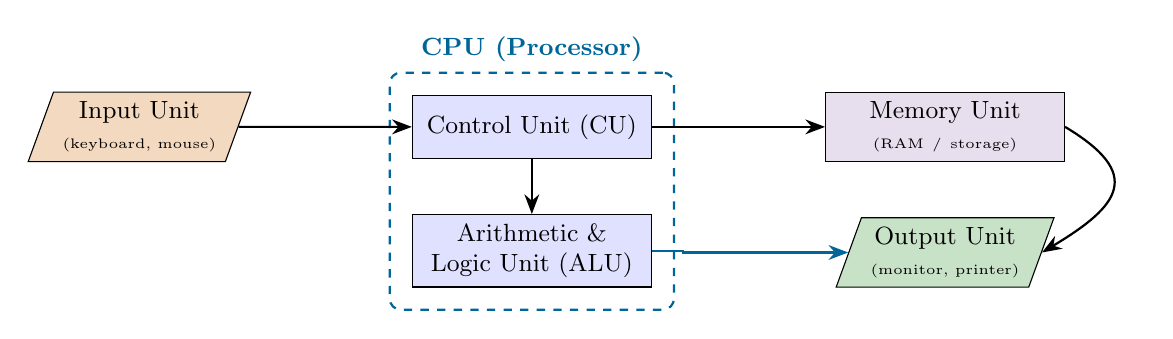
\begin{tikzpicture}[every node/.style={font=\small}, node distance=1.1cm]
        % Input
        \node[io, fill=cOrange!25] (input) {Input Unit\\ \tiny(keyboard, mouse)};
        % CPU box contents
        \node[process, right=2.2cm of input, fill=blue!12] (cu) {Control Unit (CU)};
        \node[process, below=0.7cm of cu, fill=blue!12] (alu) {Arithmetic \& Logic Unit (ALU)};
        % memory
        \node[process, right=2.2cm of cu, fill=cPurple!15] (mem) {Memory Unit\\ \tiny(RAM / storage)};
        % output
        \node[io, below=0.7cm of mem, fill=cGreen!25] (output) {Output Unit\\ \tiny(monitor, printer)};

        % CPU dashed box
        \begin{scope}[on background layer]
            \node[draw=cAccent, thick, dashed, rounded corners, fit=(cu)(alu), inner sep=8pt, label={[cAccent]above:\textbf{CPU (Processor)}}] (cpu) {};
        \end{scope}

        % arrows
        \draw[flowarrow] (input) -- (cu.west);
        \draw[flowarrow] (cu) -- (alu);
        \draw[flowarrow] (cu.east) -- (mem.west);
        \draw[flowarrow] (mem.east) .. controls +(1,-0.6) and +(1,0.6) .. (output.east);
        \draw[flowarrow, cAccent] (alu.east) -- ++(0.4,0) |- (output.west);
    \end{tikzpicture}
    \vspace{0.2cm}
    \begin{itemize}\small
        \item \textbf{CPU} = ``brain''. \textbf{CU} directs traffic; \textbf{ALU} does the maths \& comparisons.
        \item \textbf{Memory} temporarily holds data \& instructions the CPU is working on.
    \end{itemize}
\end{frame}

\begin{frame}{Hardware vs.\ Software \& Types of Memory}
    \begin{columns}[T]
        \begin{column}{0.5\textwidth}
            \begin{block}{Hardware}
                The physical parts you can \emph{touch} --- CPU, RAM, hard disk, keyboard, monitor.
            \end{block}
            \begin{block}{Software}
                The \emph{programs} (instructions) that tell the hardware what to do --- e.g.\ Windows, a game, a C program.
            \end{block}
        \end{column}
        \begin{column}{0.5\textwidth}
            \begin{block}{Primary Memory (fast, temporary)}
                \begin{itemize}\small
                    \item \textbf{RAM} --- working memory, lost when power is off (volatile).
                    \item \textbf{ROM} --- read-only, permanent start-up instructions.
                \end{itemize}
            \end{block}
            \begin{block}{Secondary Memory (slow, permanent)}
                \begin{itemize}\small
                    \item Hard disk, SSD, USB drive --- stores files even without power.
                \end{itemize}
            \end{block}
        \end{column}
    \end{columns}
\end{frame}

% =================================================================
\section{Evolution of Operating Systems}
% =================================================================
\begin{frame}{What is an Operating System (OS)?}
    \begin{block}{Operating System}
        An OS is the \textbf{master software} that manages the hardware and gives other programs
        a place to run. It is the bridge between \textbf{you}, the \textbf{programs}, and the \textbf{hardware}.
    \end{block}
    \centering
    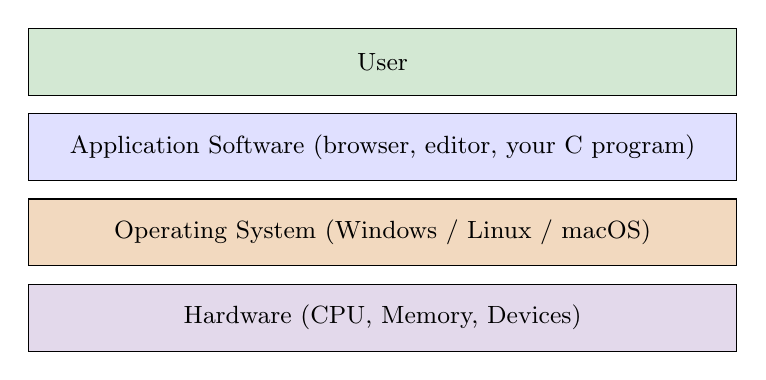
\begin{tikzpicture}[layer/.style={rectangle, draw=black, font=\small, minimum height=0.85cm, minimum width=9cm, text centered}]
        \node[layer, fill=cGreen!20] (user)  {User};
        \node[layer, fill=blue!12, below=0.22cm of user] (app)   {Application Software (browser, editor, your C program)};
        \node[layer, fill=cOrange!25, below=0.22cm of app] (os)    {Operating System (Windows / Linux / macOS)};
        \node[layer, fill=cPurple!18, below=0.22cm of os]  (hw)    {Hardware (CPU, Memory, Devices)};
    \end{tikzpicture}
    \vspace{0.15cm}

    \footnotesize Examples of tasks: managing memory, running programs, handling files, controlling devices.
\end{frame}

\begin{frame}{Evolution of Operating Systems: A Timeline}
    \centering
    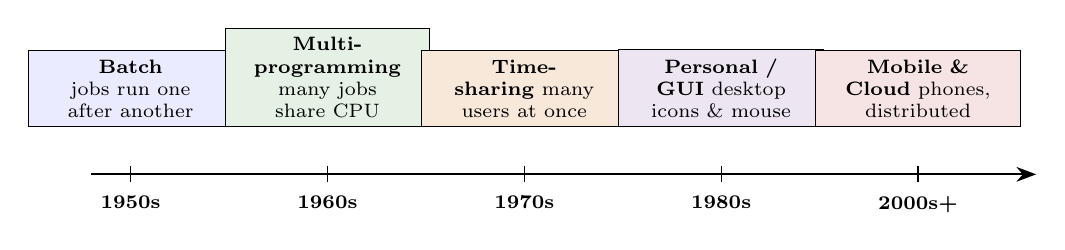
\begin{tikzpicture}[every node/.style={font=\scriptsize}]
        % timeline
        \draw[flowarrow, thick] (0,0) -- (12,0);
        \foreach \x/\yr in {0.5/1950s, 3/1960s, 5.5/1970s, 8/1980s, 10.5/2000s+} {
            \draw (\x,0.1) -- (\x,-0.1);
            \node[below] at (\x,-0.15) {\textbf{\yr}};
        }
        % milestones (alternate up/down)
        \node[process, fill=blue!8,   text width=2.2cm, above=0.6cm] at (0.5,0)  {\textbf{Batch}\\ jobs run one after another};
        \node[process, fill=cGreen!12,text width=2.2cm, above=0.6cm] at (3,0)    {\textbf{Multi-\\programming} many jobs share CPU};
        \node[process, fill=cOrange!15,text width=2.2cm, above=0.6cm] at (5.5,0) {\textbf{Time-\\sharing} many users at once};
        \node[process, fill=cPurple!12,text width=2.2cm, above=0.6cm] at (8,0)   {\textbf{Personal / GUI} desktop icons \& mouse};
        \node[process, fill=cRed!12,  text width=2.2cm, above=0.6cm] at (10.5,0) {\textbf{Mobile \& Cloud} phones, distributed};
    \end{tikzpicture}
    \vspace{0.4cm}
    \begin{itemize}\small
        \item Each stage made the computer \textbf{easier to use} and able to do \textbf{more at once}.
        \item Modern OSes let many programs and users run \emph{simultaneously} on the same machine.
    \end{itemize}
\end{frame}

% =================================================================
\section{Machine, Assembly \& High-Level Languages}
% =================================================================
\begin{frame}{Levels of Programming Languages}
    \centering
    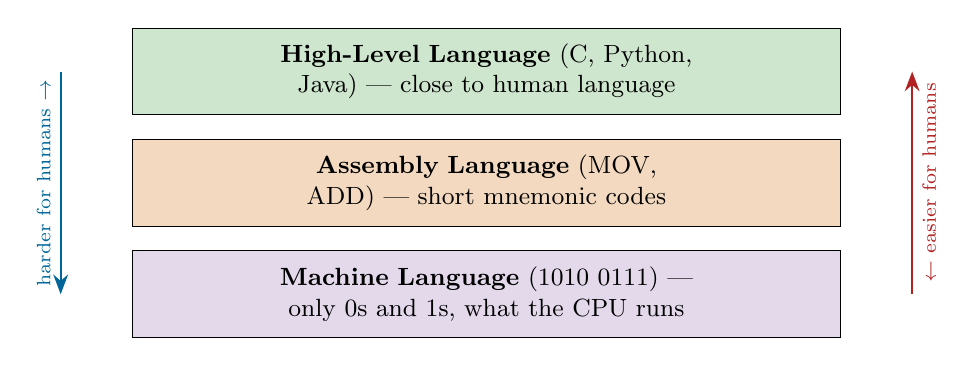
\begin{tikzpicture}[every node/.style={font=\small, text centered},
        lang/.style={rectangle, draw=black, minimum width=9cm, minimum height=1.1cm, text width=8.4cm, align=center}]
        \node[lang, fill=cGreen!22] (hl)
            {\textbf{High-Level Language} (C, Python, Java) --- close to human language};
        \node[lang, fill=cOrange!25, below=0.3cm of hl] (asm)
            {\textbf{Assembly Language} (MOV, ADD) --- short mnemonic codes};
        \node[lang, fill=cPurple!18, below=0.3cm of asm] (mc)
            {\textbf{Machine Language} (1010 0111) --- only 0s and 1s, what the CPU runs};
        \draw[flowarrow, cAccent, thick] ($(hl.west)+(-0.9,0)$) -- ($(mc.west)+(-0.9,0)$)
            node[midway, left, rotate=90, anchor=south, font=\scriptsize] {harder for humans $\rightarrow$};
        \draw[flowarrow, cRed, thick] ($(mc.east)+(0.9,0)$) -- ($(hl.east)+(0.9,0)$)
            node[midway, right, rotate=90, anchor=north, font=\scriptsize] {$\leftarrow$ easier for humans};
    \end{tikzpicture}
    \vspace{0.3cm}
    \begin{itemize}\small
        \item The CPU understands \textbf{only} machine language (binary).
        \item We write in a high-level language; a \textbf{translator} converts it to machine code.
    \end{itemize}
\end{frame}

\begin{frame}{Comparing the Three Levels}
    \renewcommand{\arraystretch}{1.4}
    \centering
    \begin{tabular}{@{}p{2.4cm}p{3.4cm}p{3.6cm}@{}}
        \toprule
        \textbf{Feature} & \textbf{Human friendliness} & \textbf{Example (add 2 numbers)} \\
        \midrule
        Machine   & Very hard (all 0/1)          & \texttt{10110000 01100001} \\
        Assembly  & Hard (mnemonics)             & \texttt{MOV AL, 61h}\quad \texttt{ADD AL, BL} \\
        High-level& Easy (English-like)          & \texttt{c = a + b;} \\
        \bottomrule
    \end{tabular}
    \vspace{0.4cm}
    \begin{block}{Key idea}
        High-level languages like \textbf{C} let us write \emph{one} readable line instead of many cryptic machine instructions --- and the same C program can run on many different machines.
    \end{block}
\end{frame}

% =================================================================
\section{Software \& Hardware Trends; Programming Methodologies}
% =================================================================
\begin{frame}{Key Software \& Hardware Trends}
    \begin{columns}[T]
        \begin{column}{0.5\textwidth}
            \begin{block}{Hardware trends}
                \begin{itemize}\small
                    \item \textbf{Moore's Law}: transistor count roughly doubles $\sim$every 2 years $\rightarrow$ faster, cheaper chips.
                    \item Multi-core CPUs, GPUs.
                    \item Smaller \& mobile: phones, embedded, IoT.
                    \item Cloud data-centres provide computing ``on tap''.
                \end{itemize}
            \end{block}
        \end{column}
        \begin{column}{0.5\textwidth}
            \begin{block}{Software trends}
                \begin{itemize}\small
                    \item Open-source software \& reusable libraries.
                    \item Mobile apps and web applications.
                    \item Artificial Intelligence \& data science.
                    \item Higher-level, safer languages built \emph{on top of} C.
                \end{itemize}
            \end{block}
        \end{column}
    \end{columns}
    \vspace{0.2cm}
    \footnotesize\centering
    Hardware gets faster and cheaper; software gets smarter and more connected --- and \textbf{C} sits underneath much of it.
\end{frame}

\begin{frame}{Procedural vs.\ Object-Oriented Programming}
    \begin{columns}[T]
        \begin{column}{0.5\textwidth}
            \begin{block}{Procedural (e.g.\ C)}
                Program = a sequence of \textbf{procedures / functions} that operate on data.
                \begin{itemize}\small
                    \item Think: a \emph{recipe} --- do step 1, then 2, then 3.
                    \item Data and functions are separate.
                \end{itemize}
            \end{block}
            \centering
            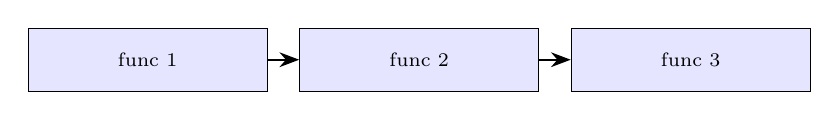
\begin{tikzpicture}[font=\scriptsize, node distance=0.4cm]
                \node[process, fill=blue!10, minimum width=1.4cm] (f1){func 1};
                \node[process, fill=blue!10, minimum width=1.4cm, right=of f1] (f2){func 2};
                \node[process, fill=blue!10, minimum width=1.4cm, right=of f2] (f3){func 3};
                \draw[flowarrow](f1)--(f2); \draw[flowarrow](f2)--(f3);
            \end{tikzpicture}
        \end{column}
        \begin{column}{0.5\textwidth}
            \begin{block}{Object-Oriented (e.g.\ C++, Java)}
                Program = a set of \textbf{objects} that bundle data \emph{and} the functions acting on it.
                \begin{itemize}\small
                    \item Think: real-world \emph{objects} (a Car that can \texttt{start()}, \texttt{stop()}).
                    \item Ideas: class, object, inheritance.
                \end{itemize}
            \end{block}
            \centering
            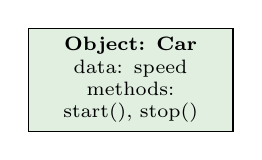
\begin{tikzpicture}[font=\scriptsize]
                \node[process, fill=cGreen!14, text width=2cm] (obj)
                    {\textbf{Object: Car}\\ data: speed\\ methods: start(), stop()};
            \end{tikzpicture}
        \end{column}
    \end{columns}
    \vspace{0.15cm}
    \footnotesize\centering In this course we focus on the \textbf{procedural} style using \textbf{C}.
\end{frame}

% =================================================================
\section{Program Development in C}
% =================================================================
\begin{frame}{Why C?}
    \begin{columns}[T]
        \begin{column}{0.55\textwidth}
            \begin{itemize}
                \item Created by \textbf{Dennis Ritchie} at Bell Labs (early 1970s).
                \item \textbf{Powerful} yet \textbf{small} --- close to the hardware but readable.
                \item The ``mother language'': Linux, databases, and parts of Windows are written in C.
                \item Learning C teaches you how a computer \emph{really} works.
            \end{itemize}
        \end{column}
        \begin{column}{0.45\textwidth}
            \begin{block}{C is a great first language because}
                \begin{itemize}\small
                    \item It is \textbf{fast}.
                    \item It is used \textbf{everywhere}.
                    \item Its ideas carry over to C++, Java, Python, \dots
                \end{itemize}
            \end{block}
        \end{column}
    \end{columns}
\end{frame}

\begin{frame}{From Source Code to Running Program}
    \centering
    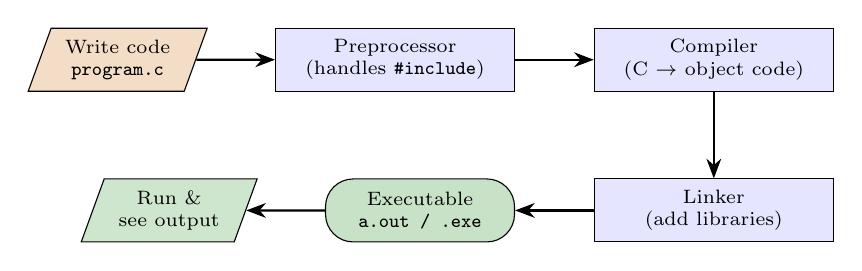
\begin{tikzpicture}[every node/.style={font=\scriptsize}, node distance=0.7cm and 1.0cm]
        \node[io, fill=cOrange!22] (edit) {Write code\\ \texttt{program.c}};
        \node[process, right=of edit, fill=blue!10] (pre) {Preprocessor\\ (handles \texttt{\#include})};
        \node[process, right=of pre, fill=blue!10]  (comp) {Compiler\\ (C $\rightarrow$ object code)};
        \node[process, below=1.1cm of comp, fill=blue!10] (link) {Linker\\ (add libraries)};
        \node[startstop, left=of link, fill=cGreen!25] (exe) {Executable\\ \texttt{a.out / .exe}};
        \node[io, left=of exe, fill=cGreen!22] (run) {Run \&\\ see output};

        \draw[flowarrow] (edit) -- (pre);
        \draw[flowarrow] (pre) -- (comp);
        \draw[flowarrow] (comp) -- (link);
        \draw[flowarrow] (link) -- (exe);
        \draw[flowarrow] (exe) -- (run);
    \end{tikzpicture}
    \vspace{0.3cm}
    \begin{block}{One command does it all (using GCC)}
        \texttt{gcc\ program.c\ -o\ program} \quad then \quad \texttt{./program}
    \end{block}
    \footnotesize If the compiler reports \textbf{errors}, fix them and compile again --- this ``edit $\rightarrow$ compile $\rightarrow$ run'' loop is normal!
\end{frame}

\begin{frame}[fragile]{Your First C Program}
\begin{lstlisting}
#include <stdio.h>          /* bring in input/output library */

int main(void)              /* execution starts here */
{
    printf("Hello, World!\n");   /* print a message */
    return 0;                    /* 0 = success */
}
\end{lstlisting}
    \begin{columns}[T]
        \begin{column}{0.5\textwidth}
            \begin{itemize}\small
                \item \texttt{\#include <stdio.h>} --- loads printf/scanf.
                \item \texttt{int main(void)} --- every C program starts in \texttt{main}.
                \item \texttt{\{ \dots \}} --- the body of the function.
            \end{itemize}
        \end{column}
        \begin{column}{0.5\textwidth}
            \begin{itemize}\small
                \item \texttt{printf(\dots)} --- prints text; \texttt{\textbackslash n} = new line.
                \item Every statement ends with a \textbf{semicolon} \texttt{;}
                \item \texttt{return 0;} --- tells the OS all went well.
            \end{itemize}
        \end{column}
    \end{columns}
    \vspace{0.15cm}
    \centering\footnotesize\textbf{Output:}\; \fbox{\texttt{Hello, World!}}
\end{frame}

% =================================================================
\section{Structured Programming: Algorithms \& Pseudo-code}
% =================================================================
\begin{frame}{Structured Programming}
    \begin{block}{Idea}
        Build every program from just \textbf{three} basic control structures. This keeps code
        clear, correct, and easy to read (no ``spaghetti'' jumps).
    \end{block}
    \centering
    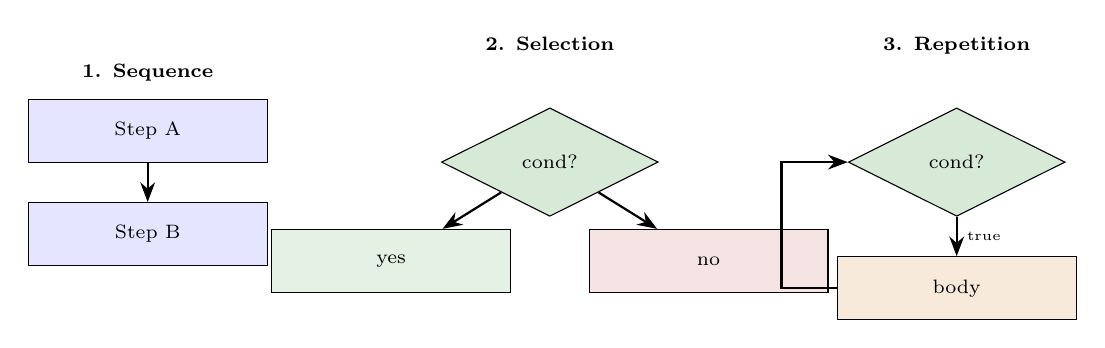
\begin{tikzpicture}[font=\scriptsize, node distance=0.5cm]
        % sequence
        \node[process, fill=blue!10, minimum width=1.6cm] (s1){Step A};
        \node[process, fill=blue!10, minimum width=1.6cm, below=of s1] (s2){Step B};
        \draw[flowarrow](s1)--(s2);
        \node[above=0.1cm of s1]{\textbf{1. Sequence}};
        % selection
        \node[decision, right=2.2cm of s1, yshift=-0.4cm] (d){cond?};
        \node[process, fill=cGreen!12, below left=0.5cm and -0.2cm of d, minimum width=1.2cm](y){yes};
        \node[process, fill=cRed!12, below right=0.5cm and -0.2cm of d, minimum width=1.2cm](n){no};
        \draw[flowarrow](d)--(y); \draw[flowarrow](d)--(n);
        \node[above=0.6cm of d]{\textbf{2. Selection}};
        % loop
        \node[decision, right=2.4cm of d] (l){cond?};
        \node[process, fill=cOrange!14, below=0.5cm of l, minimum width=1.4cm](body){body};
        \draw[flowarrow](l) -- node[right,font=\tiny]{true} (body);
        \draw[flowarrow](body.west) -- ++(-0.7,0) |- (l.west);
        \node[above=0.55cm of l]{\textbf{3. Repetition}};
    \end{tikzpicture}
    \vspace{0.2cm}
    \footnotesize\centering Sequence (do in order) \; $\bullet$ \; Selection (choose) \; $\bullet$ \; Repetition (loop).
\end{frame}

\begin{frame}[fragile]{Algorithm and Pseudo-code}
    \begin{columns}[T]
        \begin{column}{0.5\textwidth}
            \begin{block}{Algorithm}
                A finite, step-by-step procedure to solve a problem --- \emph{before} writing any code.
            \end{block}
            \textbf{Algorithm: add two numbers}
            \begin{enumerate}\small
                \item Start
                \item Read two numbers \texttt{a} and \texttt{b}
                \item Compute \texttt{sum = a + b}
                \item Display \texttt{sum}
                \item Stop
            \end{enumerate}
        \end{column}
        \begin{column}{0.5\textwidth}
            \begin{block}{Pseudo-code}
                An informal, English-like sketch of the code --- language independent.
            \end{block}
\begin{semiverbatim}\small
BEGIN
   INPUT a, b
   sum \(\leftarrow\) a + b
   OUTPUT sum
END
\end{semiverbatim}
            \vspace{0.1cm}
            \footnotesize Good pseudo-code translates almost line-by-line into C.
        \end{column}
    \end{columns}
\end{frame}

\begin{frame}{Flowchart Symbols You Should Know}
    \centering
    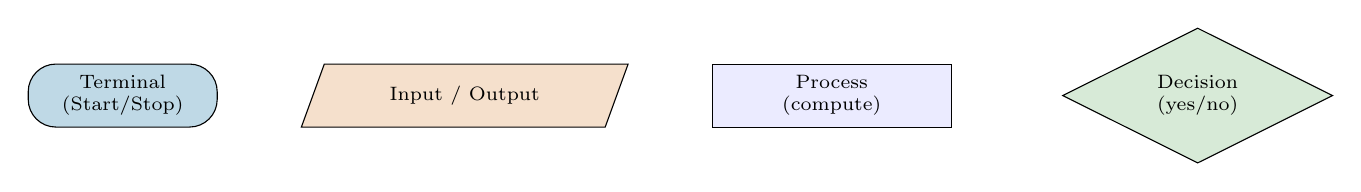
\begin{tikzpicture}[every node/.style={font=\scriptsize, text centered}, node distance=0.6cm]
        \node[startstop] (t){Terminal\\(Start/Stop)};
        \node[io, right=1.2cm of t] (io){Input / Output};
        \node[process, right=1.2cm of io] (p){Process\\(compute)};
        \node[decision, right=1.4cm of p] (d){Decision\\(yes/no)};
    \end{tikzpicture}
    \vspace{0.5cm}
    \begin{block}{Flowchart: add two numbers}
        \centering
        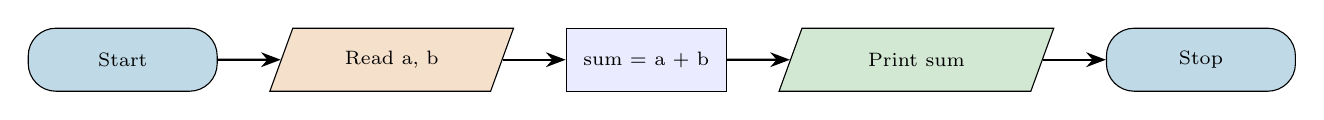
\begin{tikzpicture}[every node/.style={font=\scriptsize}, node distance=0.8cm]
            \node[startstop] (start){Start};
            \node[io, right=of start, fill=cOrange!20] (read){Read a, b};
            \node[process, right=of read, minimum width=1.8cm, text width=1.8cm] (calc){sum = a + b};
            \node[io, right=of calc, fill=cGreen!20] (print){Print sum};
            \node[startstop, right=of print] (stop){Stop};
            \draw[flowarrow](start)--(read);
            \draw[flowarrow](read)--(calc);
            \draw[flowarrow](calc)--(print);
            \draw[flowarrow](print)--(stop);
        \end{tikzpicture}
    \end{block}
\end{frame}

% =================================================================
\section{The C Standard Library}
% =================================================================
\begin{frame}{The C Standard Library}
    \begin{block}{What is it?}
        A ready-made collection of \textbf{functions} that come with C, so you don't reinvent the wheel.
        You get access to them with \texttt{\#include <header.h>}.
    \end{block}
    \renewcommand{\arraystretch}{1.3}
    \centering
    \begin{tabular}{@{}llp{5.2cm}@{}}
        \toprule
        \textbf{Header} & \textbf{Purpose} & \textbf{Example functions} \\
        \midrule
        \texttt{stdio.h}  & input / output      & \texttt{printf}, \texttt{scanf}, \texttt{getchar} \\
        \texttt{stdlib.h} & general utilities   & \texttt{malloc}, \texttt{rand}, \texttt{abs}, \texttt{atoi} \\
        \texttt{math.h}   & mathematics         & \texttt{sqrt}, \texttt{pow}, \texttt{sin}, \texttt{ceil} \\
        \texttt{string.h} & text handling       & \texttt{strlen}, \texttt{strcpy}, \texttt{strcmp} \\
        \texttt{ctype.h}  & character tests     & \texttt{isdigit}, \texttt{toupper} \\
        \bottomrule
    \end{tabular}
    \vspace{0.2cm}
    \footnotesize\centering e.g.\ \texttt{\#include <math.h>} then \texttt{y = sqrt(25.0);} gives \texttt{y = 5.0}.
\end{frame}

% =================================================================
\section{Data Types in C}
% =================================================================
\begin{frame}{Variables and Data Types}
    \begin{block}{Variable}
        A \textbf{named box} in memory that stores a value. You must declare its \emph{type} first:
        \texttt{int age = 20;}
    \end{block}
    \centering
    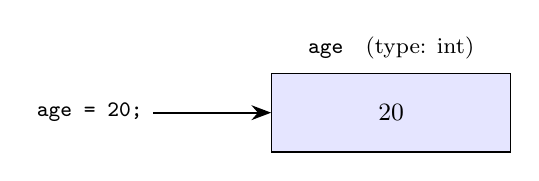
\begin{tikzpicture}[font=\small]
        \node[process, minimum width=1.6cm, minimum height=1cm, fill=blue!10] (box) {20};
        \node[above=0.05cm of box, font=\footnotesize] {\texttt{age} \; (type: int)};
        \draw[flowarrow] ($(box.west)+(-1.5,0)$) node[left, font=\footnotesize]{\texttt{age = 20;}} -- (box.west);
    \end{tikzpicture}
    \vspace{0.2cm}
    \begin{itemize}\small
        \item The \textbf{type} decides what values fit and how much memory is used.
        \item Choose the smallest type that comfortably holds your data.
    \end{itemize}
\end{frame}

\begin{frame}{The Basic Data Types}
    \renewcommand{\arraystretch}{1.35}
    \centering
    \begin{tabular}{@{}llll@{}}
        \toprule
        \textbf{Type} & \textbf{Stores} & \textbf{Typical size} & \textbf{Example} \\
        \midrule
        \texttt{int}    & whole numbers            & 4 bytes & \texttt{int n = 42;} \\
        \texttt{float}  & real numbers (decimals)  & 4 bytes & \texttt{float g = 9.8f;} \\
        \texttt{double} & real numbers (more precise) & 8 bytes & \texttt{double pi = 3.14159;} \\
        \texttt{char}   & a single character       & 1 byte  & \texttt{char grade = 'A';} \\
        \bottomrule
    \end{tabular}
    \vspace{0.3cm}
    \begin{columns}[T]
        \begin{column}{0.5\textwidth}
            \begin{block}{Modifiers}
                \small \texttt{short}, \texttt{long}, \texttt{unsigned} adjust range/size, e.g.\ \texttt{unsigned int} (no negatives), \texttt{long int} (bigger).
            \end{block}
        \end{column}
        \begin{column}{0.5\textwidth}
            \begin{block}{A character is a small number}
                \small \texttt{'A'} is stored as the integer \texttt{65} (its ASCII code).
            \end{block}
        \end{column}
    \end{columns}
\end{frame}

% =================================================================
\section{Arithmetic Operators}
% =================================================================
\begin{frame}{Arithmetic Operators}
    \renewcommand{\arraystretch}{1.35}
    \centering
    \begin{tabular}{@{}cllc@{}}
        \toprule
        \textbf{Operator} & \textbf{Meaning} & \textbf{Example} & \textbf{Result} \\
        \midrule
        \texttt{+} & addition        & \texttt{7 + 3}  & \texttt{10} \\
        \texttt{-} & subtraction     & \texttt{7 - 3}  & \texttt{4}  \\
        \texttt{*} & multiplication  & \texttt{7 * 3}  & \texttt{21} \\
        \texttt{/} & division        & \texttt{7 / 3}  & \texttt{2}  (integer!) \\
        \texttt{\%} & modulus (remainder) & \texttt{7 \% 3} & \texttt{1} \\
        \bottomrule
    \end{tabular}
    \vspace{0.3cm}
    \begin{block}{\textbf{Beginner trap:} integer division}
        \small \texttt{7 / 3} gives \texttt{2}, \emph{not} 2.33, because both are integers.
        Use \texttt{7.0 / 3} to get \texttt{2.333\ldots} \; The \texttt{\%} operator works only on integers.
    \end{block}
\end{frame}

\begin{frame}{Operator Precedence (Order of Operations)}
    \begin{columns}[T]
        \begin{column}{0.52\textwidth}
            \begin{itemize}
                \item C follows maths-like precedence: \\[2pt]
                \centering \texttt{*}\; \texttt{/}\; \texttt{\%} \; \textbf{before} \; \texttt{+}\; \texttt{-}
                \item Same level $\rightarrow$ left to right.
                \item Use \textbf{parentheses} to be explicit and clear.
            \end{itemize}
            \vspace{0.3cm}
            \begin{block}{Example}
                \small
                \texttt{2 + 3 * 4} \; $\rightarrow$ \; \texttt{2 + 12} \; $\rightarrow$ \; \texttt{14} \\
                \texttt{(2 + 3) * 4} \; $\rightarrow$ \; \texttt{20}
            \end{block}
        \end{column}
        \begin{column}{0.48\textwidth}
            \begin{block}{Assignment \& shortcuts}
                \small
                \begin{itemize}
                    \item \texttt{x = 5;} stores 5 in \texttt{x}.
                    \item \texttt{x += 2;} means \texttt{x = x + 2;}
                    \item \texttt{x++;} increases \texttt{x} by 1.
                    \item \texttt{x{-}{-};} decreases \texttt{x} by 1.
                \end{itemize}
            \end{block}
        \end{column}
    \end{columns}
\end{frame}

% =================================================================
\section{Control Structures}
% =================================================================
\begin{frame}[fragile]{Making Decisions: \texttt{if} / \texttt{if-else}}
    \begin{columns}[T]
        \begin{column}{0.55\textwidth}
\begin{lstlisting}
if (marks >= 40) {
    printf("Pass\n");
} else {
    printf("Fail\n");
}
\end{lstlisting}
            \begin{itemize}\small
                \item The condition in \texttt{( )} is either \textbf{true} or \textbf{false}.
                \item Comparisons: \texttt{==}\; \texttt{!=}\; \texttt{<}\; \texttt{>}\; \texttt{<=}\; \texttt{>=}
                \item \textbf{Trap:} \texttt{==} tests equality; \texttt{=} \emph{assigns}!
            \end{itemize}
        \end{column}
        \begin{column}{0.45\textwidth}
            \centering
            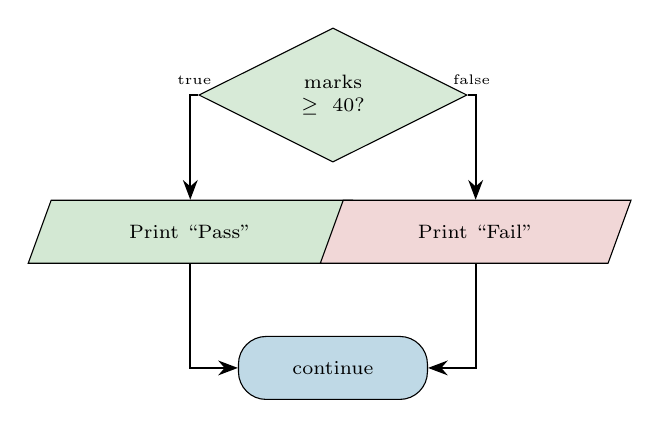
\begin{tikzpicture}[font=\scriptsize, node distance=0.55cm]
                \node[decision] (d){marks \\ $\geq 40$?};
                \node[io, below left=0.9cm and 0.55cm of d, fill=cGreen!20] (p){Print ``Pass''};
                \node[io, below right=0.9cm and 0.55cm of d, fill=cRed!18] (f){Print ``Fail''};
                \node[startstop, below=2.2cm of d] (m){continue};
                \draw[flowarrow] (d.west) -| node[near start,above,font=\tiny]{true} (p);
                \draw[flowarrow] (d.east) -| node[near start,above,font=\tiny]{false} (f);
                \draw[flowarrow] (p) |- (m);
                \draw[flowarrow] (f) |- (m);
            \end{tikzpicture}
        \end{column}
    \end{columns}
\end{frame}

\begin{frame}[fragile]{Choosing Among Many: \texttt{switch}}
    \begin{columns}[T]
        \begin{column}{0.55\textwidth}
\begin{lstlisting}
switch (choice) {
    case 1:
        printf("Add\n");
        break;
    case 2:
        printf("Subtract\n");
        break;
    default:
        printf("Invalid\n");
}
\end{lstlisting}
        \end{column}
        \begin{column}{0.45\textwidth}
            \begin{itemize}\small
                \item Compares one variable against several \texttt{case} values.
                \item \texttt{break;} stops ``falling through'' to the next case --- \textbf{don't forget it}.
                \item \texttt{default:} runs if nothing else matches.
                \item Cleaner than a long \texttt{if--else if} chain.
            \end{itemize}
            \begin{block}{Note}
                \small \texttt{case} labels must be constant integers or characters (e.g.\ \texttt{1}, \texttt{'A'}).
            \end{block}
        \end{column}
    \end{columns}
\end{frame}

\begin{frame}[fragile]{Loops: \texttt{while} and \texttt{do--while}}
    \begin{columns}[T]
        \begin{column}{0.5\textwidth}
            \textbf{\texttt{while}} --- test \emph{first}, may run 0 times:
\begin{lstlisting}
int i = 1;
while (i <= 5) {
    printf("%d ", i);
    i++;
}
\end{lstlisting}
            \centering
            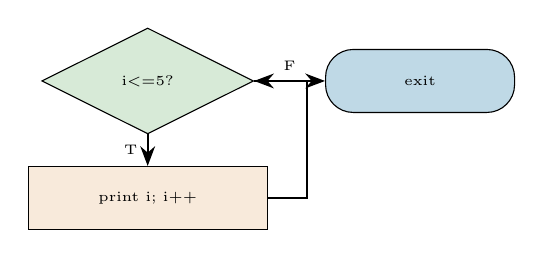
\begin{tikzpicture}[font=\tiny, node distance=0.4cm]
                \node[decision] (c){i<=5?};
                \node[process, below=of c, fill=cOrange!14](b){print i; i++};
                \node[startstop, right=0.9cm of c](x){exit};
                \draw[flowarrow](c)-- node[left]{T}(b);
                \draw[flowarrow](c)-- node[above]{F}(x);
                \draw[flowarrow](b.east)--++(0.5,0)|-(c.east);
            \end{tikzpicture}
        \end{column}
        \begin{column}{0.5\textwidth}
            \textbf{\texttt{do--while}} --- test \emph{after}, runs $\geq 1$ time:
\begin{lstlisting}
int i = 1;
do {
    printf("%d ", i);
    i++;
} while (i <= 5);
\end{lstlisting}
            \centering
            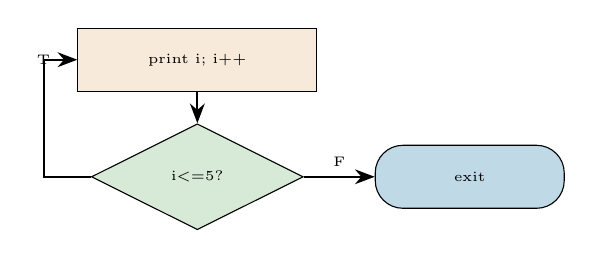
\begin{tikzpicture}[font=\tiny, node distance=0.4cm]
                \node[process, fill=cOrange!14](b){print i; i++};
                \node[decision, below=of b] (c){i<=5?};
                \node[startstop, right=0.9cm of c](x){exit};
                \draw[flowarrow](b)--(c);
                \draw[flowarrow](c)-- node[above]{F}(x);
                \draw[flowarrow](c.west)--++(-0.6,0)|-(b.west) node[near end,left]{T};
            \end{tikzpicture}
        \end{column}
    \end{columns}
    \vspace{0.1cm}
    \centering\footnotesize Both print \fbox{\texttt{1 2 3 4 5}}. Use \texttt{do--while} when the body must run at least once.
\end{frame}

\begin{frame}[fragile]{Loops: the \texttt{for} Loop}
    \begin{columns}[T]
        \begin{column}{0.55\textwidth}
\begin{lstlisting}
for (i = 1; i <= 5; i++) {
    printf("%d ", i);
}
\end{lstlisting}
            The three parts of a \texttt{for} loop:
            \begin{enumerate}\small
                \item \textbf{Init}: \texttt{i = 1} --- runs once at the start.
                \item \textbf{Condition}: \texttt{i <= 5} --- checked before each pass.
                \item \textbf{Update}: \texttt{i++} --- runs after each pass.
            \end{enumerate}
        \end{column}
        \begin{column}{0.45\textwidth}
            \centering
            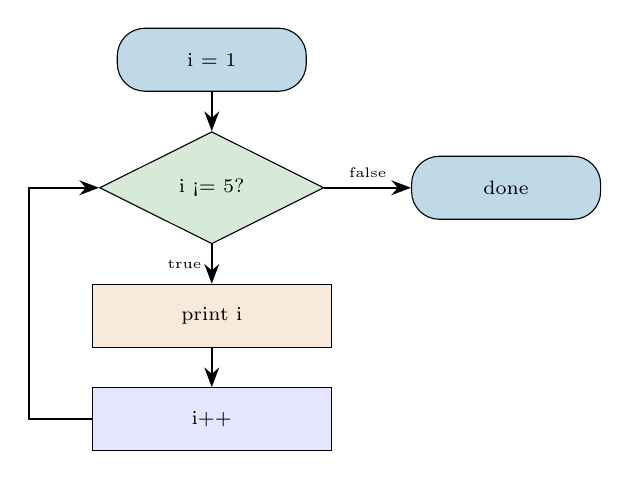
\begin{tikzpicture}[font=\scriptsize, node distance=0.5cm]
                \node[startstop] (init){i = 1};
                \node[decision, below=of init] (cond){i <= 5?};
                \node[process, below=of cond, fill=cOrange!14] (body){print i};
                \node[process, below=of body, fill=blue!10] (upd){i++};
                \node[startstop, right=1.1cm of cond] (done){done};
                \draw[flowarrow](init)--(cond);
                \draw[flowarrow](cond)-- node[left,font=\tiny]{true}(body);
                \draw[flowarrow](cond)-- node[above,font=\tiny]{false}(done);
                \draw[flowarrow](body)--(upd);
                \draw[flowarrow](upd.west)--++(-0.8,0)|-(cond.west);
            \end{tikzpicture}
        \end{column}
    \end{columns}
    \vspace{0.1cm}
    \centering\footnotesize A \texttt{for} loop is a compact \texttt{while} loop --- best when you know the count in advance.
\end{frame}

\begin{frame}[fragile]{\texttt{break} and \texttt{continue}}
    \begin{columns}[T]
        \begin{column}{0.5\textwidth}
            \textbf{\texttt{break}} --- exit the loop immediately.
\begin{lstlisting}
for (i = 1; i <= 10; i++) {
    if (i == 4) break;
    printf("%d ", i);
}
// prints: 1 2 3
\end{lstlisting}
        \end{column}
        \begin{column}{0.5\textwidth}
            \textbf{\texttt{continue}} --- skip to the next iteration.
\begin{lstlisting}
for (i = 1; i <= 5; i++) {
    if (i == 3) continue;
    printf("%d ", i);
}
// prints: 1 2 4 5
\end{lstlisting}
        \end{column}
    \end{columns}
    \vspace{0.2cm}
    \begin{block}{Remember}
        \small \texttt{break} \textbf{leaves} the loop; \texttt{continue} \textbf{jumps to the next round}. Both also appear inside \texttt{while}/\texttt{do--while}; \texttt{break} additionally ends a \texttt{switch} case.
    \end{block}
\end{frame}

% =================================================================
\section{Formatted Input and Output}
% =================================================================
\begin{frame}[fragile]{Output with \texttt{printf} --- Format Specifiers}
    \renewcommand{\arraystretch}{1.3}
    \centering
    \begin{tabular}{@{}cll@{}}
        \toprule
        \textbf{Specifier} & \textbf{Used for} & \textbf{Example} \\
        \midrule
        \texttt{\%d} & integer               & \texttt{printf("\%d", 42);} $\rightarrow$ \texttt{42} \\
        \texttt{\%f} & float / double        & \texttt{printf("\%f", 3.14);} $\rightarrow$ \texttt{3.140000} \\
        \texttt{\%c} & single character      & \texttt{printf("\%c", 'A');} $\rightarrow$ \texttt{A} \\
        \texttt{\%s} & string (text)         & \texttt{printf("\%s", "Hi");} $\rightarrow$ \texttt{Hi} \\
        \bottomrule
    \end{tabular}
    \vspace{0.3cm}
    \begin{columns}[T]
        \begin{column}{0.5\textwidth}
            \begin{block}{Width \& precision}
                \small
                \texttt{\%5d} --- at least 5 columns wide.\\
                \texttt{\%.2f} --- 2 digits after the point.\\
                \texttt{printf("\%.2f", 3.14159);} $\rightarrow$ \texttt{3.14}
            \end{block}
        \end{column}
        \begin{column}{0.5\textwidth}
            \begin{block}{Escape sequences}
                \small
                \texttt{\textbackslash n} new line \quad \texttt{\textbackslash t} tab \\
                \texttt{\textbackslash\textbackslash} backslash \quad \texttt{\textbackslash"} quote
            \end{block}
        \end{column}
    \end{columns}
\end{frame}

\begin{frame}[fragile]{Input with \texttt{scanf}}
\begin{lstlisting}
int age;
printf("Enter your age: ");
scanf("%d", &age);          /* note the & (address of age) */
printf("Next year you will be %d\n", age + 1);
\end{lstlisting}
    \begin{itemize}\small
        \item \texttt{scanf} reads typed input and stores it in a variable.
        \item \textbf{Crucial:} put an \texttt{\&} (``address of'') before the variable --- \texttt{\&age}.
        \item The specifier must match the type: \texttt{\%d} int, \texttt{\%f} float, \texttt{\%c} char, \texttt{\%s} string.
    \end{itemize}
    \begin{block}{Reading several values}
        \small \texttt{scanf("\%d \%f", \&n, \&x);} reads an integer then a float.
    \end{block}
    \centering\footnotesize\textbf{Sample run:}\; \fbox{\texttt{Enter your age: 20}} $\rightarrow$ \fbox{\texttt{Next year you will be 21}}
\end{frame}

% =================================================================
\section{Simple C Programming Examples}
% =================================================================
\begin{frame}[fragile]{Example 1 --- Add Two Numbers}
\begin{lstlisting}
#include <stdio.h>

int main(void)
{
    int a, b, sum;

    printf("Enter two integers: ");
    scanf("%d %d", &a, &b);

    sum = a + b;
    printf("Sum = %d\n", sum);

    return 0;
}
\end{lstlisting}
    \centering\footnotesize
    \textbf{Run:}\; \fbox{\texttt{Enter two integers: 7 5}} $\rightarrow$ \fbox{\texttt{Sum = 12}}
\end{frame}

\begin{frame}[fragile]{Example 2 --- Even or Odd (\texttt{if--else} + \texttt{\%})}
\begin{lstlisting}
#include <stdio.h>

int main(void)
{
    int n;
    printf("Enter a number: ");
    scanf("%d", &n);

    if (n % 2 == 0)
        printf("%d is Even\n", n);
    else
        printf("%d is Odd\n", n);

    return 0;
}
\end{lstlisting}
    \centering\footnotesize \textbf{Idea:} a number is even when \texttt{n \% 2} (the remainder) is \texttt{0}.
\end{frame}

\begin{frame}[fragile]{Example 3 --- Sum of 1 to N (a \texttt{for} loop)}
    \begin{columns}[T]
        \begin{column}{0.62\textwidth}
\begin{lstlisting}
#include <stdio.h>

int main(void)
{
    int n, i, sum = 0;

    printf("Enter N: ");
    scanf("%d", &n);

    for (i = 1; i <= n; i++)
        sum += i;   /* sum = sum + i */

    printf("Sum 1..%d = %d\n", n, sum);
    return 0;
}
\end{lstlisting}
        \end{column}
        \begin{column}{0.38\textwidth}
            \begin{block}{Trace for N = 5}
                \small
                \begin{tabular}{cc}
                    \texttt{i} & \texttt{sum} \\ \hline
                    1 & 1  \\
                    2 & 3  \\
                    3 & 6  \\
                    4 & 10 \\
                    5 & 15 \\
                \end{tabular}
            \end{block}
            \centering\footnotesize Output:\\ \fbox{\texttt{Sum 1..5 = 15}}
        \end{column}
    \end{columns}
\end{frame}

\begin{frame}[fragile]{Example 4 --- Simple Calculator (\texttt{switch})}
\begin{lstlisting}
#include <stdio.h>
int main(void) {
    float a, b;  char op;
    printf("Enter: a op b  (e.g. 6 * 7): ");
    scanf("%f %c %f", &a, &op, &b);

    switch (op) {
        case '+': printf("= %.2f\n", a + b); break;
        case '-': printf("= %.2f\n", a - b); break;
        case '*': printf("= %.2f\n", a * b); break;
        case '/':
            if (b != 0) printf("= %.2f\n", a / b);
            else        printf("Cannot divide by zero!\n");
            break;
        default:  printf("Unknown operator\n");
    }
    return 0;
}
\end{lstlisting}
\end{frame}

\begin{frame}{Summary \& What Comes Next}
    \begin{columns}[T]
        \begin{column}{0.5\textwidth}
            \begin{block}{You now know}
                \begin{itemize}\small
                    \item How a computer is organized and what an OS does.
                    \item Machine / assembly / high-level languages.
                    \item How a C program is written, compiled, and run.
                    \item Data types, operators, and control structures.
                    \item Formatted input/output with \texttt{printf}/\texttt{scanf}.
                \end{itemize}
            \end{block}
        \end{column}
        \begin{column}{0.5\textwidth}
            \begin{block}{Practice makes perfect}
                \begin{itemize}\small
                    \item Type and run every example yourself.
                    \item Deliberately make errors --- read the messages.
                    \item Modify examples: change values, add features.
                \end{itemize}
            \end{block}
            \begin{block}{Coming up}
                \small Functions, arrays, strings, and pointers.
            \end{block}
        \end{column}
    \end{columns}
\end{frame}

%------------------------------------------------
\begin{frame}
    \centering
    \Huge Thank You
    \vspace{0.5cm}

    \normalsize Questions?
\end{frame}

%------------------------------------------------
\end{document}
